
\chapter{The Factory pattern}

Now that we've covered inheritance, we're in a position to understand the next
simple-yet-ubiquitous design pattern, called \textbf{Factory}. It's a pretty
easy one to grasp. Simply put, a factory is \textit{a class whose purpose is
to instantiate objects.}

\index{new@\texttt{new}}
Up to now, we've used the \texttt{new} operator directly in order to
instantiate. If we want a new \texttt{Ballplayer} object, we \texttt{new} one
up:

\vspace{-.1in}
\begin{Verbatim}[fontsize=\small,samepage=true,frame=none]
  Ballplayer joe = new Ballplayer("Dimaggio","OF");
\end{Verbatim}
\vspace{-.1in}

\index{ballplayer@\texttt{BallplayerFactory}}
We're now going to outsource this instantiation process to a special class
called a \texttt{BallplayerFactory}. It'll seem like unnecessary wiring at
first, but there are advantages that come to light when the instantiation
process is more complicated. Our new line of code will be this:

\vspace{-.1in}
\begin{Verbatim}[fontsize=\small,samepage=true,frame=none]
  Ballplayer joe =
      BallplayerFactory.instance().create("Dimaggio","OF");
\end{Verbatim}
\vspace{-.1in}

\index{Singleton pattern}
\index{design pattern!Singleton}
\index{object-oriented}
\index{instance@\texttt{.instance()}}
The sharp-eyed reader will see the \texttt{.instance()} and wonder if this is
using the \textbf{Singleton} pattern. The answer is yes! In fact,
\textit{factories are nearly always singletons.} This is simply because
although our baseball simulator will create lots of \texttt{Ballplayer}s, it
will only need one \texttt{BallplayerFactory}.\footnote{As with all design
patterns, you should use standard nomenclature. If the word ``factory'' seems
clunky or contrived to you, I get it, but accept it as part of the OOP culture
and use it. Don't try to come up with your own synonym of ``factory'' (like
``creator'' or ``instantiator'') and use that instead, since you'll just confuse
your fellow programmers. The word ``factory,'' like the word ``singleton,'' is
baked into the software development community's consciousness, and thus serves
as an excellent terse-yet-precise communication of purpose.}

Patterns interleave and play off one another all the time. Here, we have a
factory class that uses the classic Singleton pattern:

\begin{Verbatim}[fontsize=\footnotesize,samepage=true,frame=single]
class BallplayerFactory {

    private static BallplayerFactory theInstance;
    
    public static synchronized BallplayerFactory instance() {
        if (theInstance == null) {
            theInstance = new BallplayerFactory();
        }
        return theInstance;
    }

    private BallplayerFactory() {
    }

    public Ballplayer create(String name, String position) {
        return new Ballplayer(name, position);
    }
}
\end{Verbatim}

Badda-boom.

Now I know what you're thinking. You're thinking ``wow, that's a whole lot of
code to do nothing but ``\texttt{new} up a \texttt{Ballplayer},'' which we were
doing before with one line of code and a lot less work. What's the point of
all this?''

\index{decoupling}
\index{subclass}
The answer is that oftentimes \textit{the code which needs to instantiate an
object isn't aware of what specific subtype of object it needs.} Read that
sentence again and let it sink in. This type of decoupling -- one part of the
code that directs objects to do things without being aware of subclasses, and
a different part of the code that implements subtype-specific behavior -- is
one of the important benefits a properly-designed object-oriented program can
bring.

\section[Top-down inheritance]
{\large Top-down inheritance and the Factory pattern}

\index{inheritance!top-down (interface)}
This is in fact the launch point of top-down inheritance. We've seen that with
top-down inheritance, the client code can treat all specific subtypes (like
\texttt{Cow}, \texttt{Duck}, \textit{etc.}) in exactly the same way -- in
fact, it doesn't even have to be aware that there \textit{are} any subtypes.
To the client code, all that exists are \texttt{Animal}s, and those objects
can be directed to move, make noise, or anything else.

That was all great, but one thing we didn't address was ``how do those objects
come into existence in the first place?'' Somewhere the specific subtype
\textit{has} to be mentioned in the code, or else there's no way to
``\texttt{new}'' it. How can we be blissfully ignorant of the subtypes if we're
the one who has to instantiate them?

\index{Factory pattern}
\index{design pattern!Factory}
The answer is the Factory pattern. With it, we turn over control of the actual
instantiation to the factory class, rather than burdening the client code with
it.

Suppose that our simulator is more sophisticated than the original toy example
from Chapter~\ref{ch:memoryMatters}. Different positions have different kinds
of stats: pitchers (with ``\texttt{koDominance}'') are completely different
than position players (who have \texttt{numHits} and \texttt{numAtBats}
instead). It might make sense to use an inheritance hierarchy here with
subclasses of \texttt{Ballplayer}, as shown in
Figure~\ref{ballplayerInheritance}.

\index{inheritance hierarchy}
\index{tree}
\begin{figure}[ht]
\begin{Verbatim}[fontsize=\scriptsize,samepage=true,frame=single]
class Ballplayer {
    protected String name;
    private int uni;
    private int salary;
    private String handedness;  //  "L" or "R"

    public abstract double estimatedMarketValue();
}

class Pitcher extends Ballplayer {
    private double koDominance;
    private int numKos;

    public Pitcher(String name) { this.name = name; }
    public double estimatedMarketValue() {
        return koDominance * 20000000;
    }
}

class PositionPlayer extends Ballplayer {
    private String position;
    private int numHits;
    private int numAtBats;

    public PositionPlayer(String name, String pos) {
        this.name = name;
        this.position = pos;
    }
    public double estimatedMarketValue() {
        return numHits * 100000 - numAtBats * 1000;
    }
}
\end{Verbatim}
\caption{A small inheritance hierarchy for baseball players.}
\label{ballplayerInheritance}
\end{figure}

Our factory can now instantiate \textit{the right kind} of \texttt{Ballplayer}
when it is asked to:

\begin{Verbatim}[fontsize=\small,samepage=true,frame=single]
class BallplayerFactory {
    ...

    public Ballplayer create(String name, String position) {
        if (position.equals("P")) {
            return new Pitcher(name);
        } else {
            return new PositionPlayer(name, position);
        }
    }
}
\end{Verbatim}

Depending on the position (``\texttt{P}'' for pitcher, ``\texttt{OF}'' for
outfielder, \textit{etc.}) the factory instantiates the proper subtype of
\texttt{Ballplayer} and returns it. The client code doesn't need to know
anything about those subtypes. Notice that the return value of
\texttt{.create()} is the general type \texttt{Ballplayer}, not any of the
specific types. If we later add additional subclasses, only the factory class
has to be updated, not the code that (unknowingly) uses them.

\section{Random type generation}

\index{random number generation}
In games and simulations, it's common to instantiate objects according to some
random pattern, rather than specifying each type of object deterministically.

\index{monsterFactory@\texttt{MonsterFactory}}
Imagine a fantasy-genre videogame in which the player acts as a swordsman or
Valkyrie and wanders through dungeon levels looking for monsters to slay. We
might have a \texttt{MonsterFactory} class to generate monsters as they are
encountered. Maybe on the first (and easiest) level of the game, half of the
monsters we create are \texttt{Goblin}s and the other half are
\texttt{TempleGuard}s. And both of these have ``easy'' statistics --
\textit{i.e.}, low values for \texttt{hitPoints}, \texttt{armorClass}, and
\texttt{speed}. When the player gets to level two, however, not only will the
stats of these basic creatures get buffed, but now an occasional
\texttt{Vampire} will enter the mix.

\begin{figure}
\centering
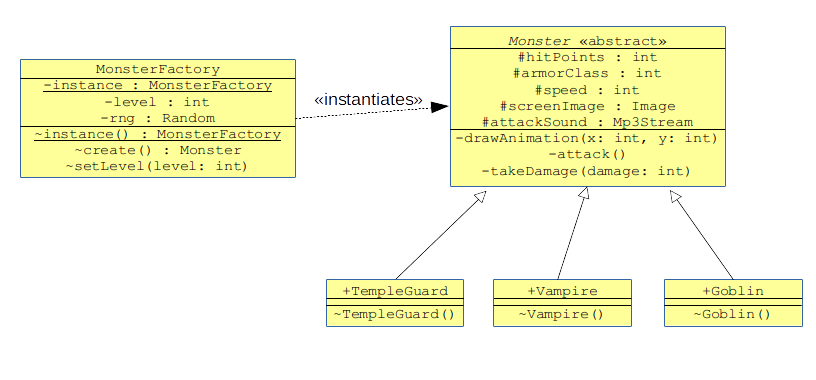
\includegraphics[width=1\textwidth]{monsterFactory.pdf}
\caption{The factory pattern in a randomly-generated setting.}
\label{fig:monsterFactory}
\end{figure}

\index{create@\texttt{.create()}}
The Factory pattern makes this easy. All we need to do is encapsulate the
functionality for creating monsters into the \texttt{.create()} method, as
shown in Figure~\ref{fig:monsterFactoryCode}. Then, whenever our program needs
to create a new bad guy, this line of code suffices:

\begin{Verbatim}[fontsize=\small,samepage=true,frame=none]
  Monster newMonster = MonsterFactory.instance().create();
\end{Verbatim}

When the player completes a level and is ready for the next challenge, our
client code simply calls:

\begin{Verbatim}[fontsize=\small,samepage=true,frame=none]
  int currLevel = MonsterFactory.instance().getLevel();
  MonsterFactory.instance().setLevel(currLevel + 1);
\end{Verbatim}

and away we go.

\index{Random.nextDouble@\texttt{Random.nextDouble()}}
\begin{figure}
\begin{Verbatim}[fontsize=\footnotesize,samepage=true,frame=single]
class MonsterFactory {
    private int level;
    private java.util.Random rng;
    
    ...singleton stuff...

    Monster create() {
        Monster m = null;
        switch (level) {
            case 1:
                double randomNumber = rng.nextDouble();
                if (randomNumber < .5) {
                    m = new Goblin();
                } else {
                    m = new TempleGuard();
                }
                m.setHitPoints(rng.nextInt(8));
                m.setArmorClass(rng.nextInt(8));
                m.setSpeed(rng.nextInt(5));
                break;
            case 2:
                double randomNumber = rng.nextDouble();
                if (randomNumber < .4) {
                    m = new Goblin();
                } else if (randomNumber < .8) {
                    m = new TempleGuard();
                } else {
                    m = new Vampire();
                }
                m.setHitPoints(rng.nextInt(8) + 5);
                m.setArmorClass(rng.nextInt(8) + 4);
                m.setSpeed(rng.nextInt(10));
                break;
        }
        return m;
    }
}
\end{Verbatim}
\caption{A factory to generate baddies randomly, based on the game's level.
(Recall the \texttt{java.util.Random} class from Section~\ref{Random} on
p.~\pageref{Random}.)}
\label{fig:monsterFactoryCode}
\end{figure}

Hopefully you're getting the gist, here: if the instantiation process for an
object is a bit complex, it makes sense to separate it into its own class.
This way, you don't have to duplicate the logic in separate places, and you
don't have to clutter your client code with a giant \texttt{switch} or
\texttt{if-else} construct right in the middle of instantiating and using an
object.

